\documentclass[tikz,border=6pt]{standalone}
\usepackage[sfdefault,lining]{FiraSans}
\usepackage{amsmath}
\usepackage{firamath-otf}
\setmathrm{Fira Sans}
\usepackage{pgfplots}
\pgfplotsset{compat=1.18}
\usetikzlibrary{arrows.meta,calc,patterns}
\definecolor{ink}{HTML}{1F2A37}\definecolor{grey}{HTML}{6B7280}\definecolor{sea}{HTML}{1D4E89}
\definecolor{accent}{HTML}{0F766E}
\newcommand{\wavecol}[2]{\definecolor{tmpwave}{wave}{#2}\colorlet{#1}[rgb]{tmpwave}}
\begin{document}

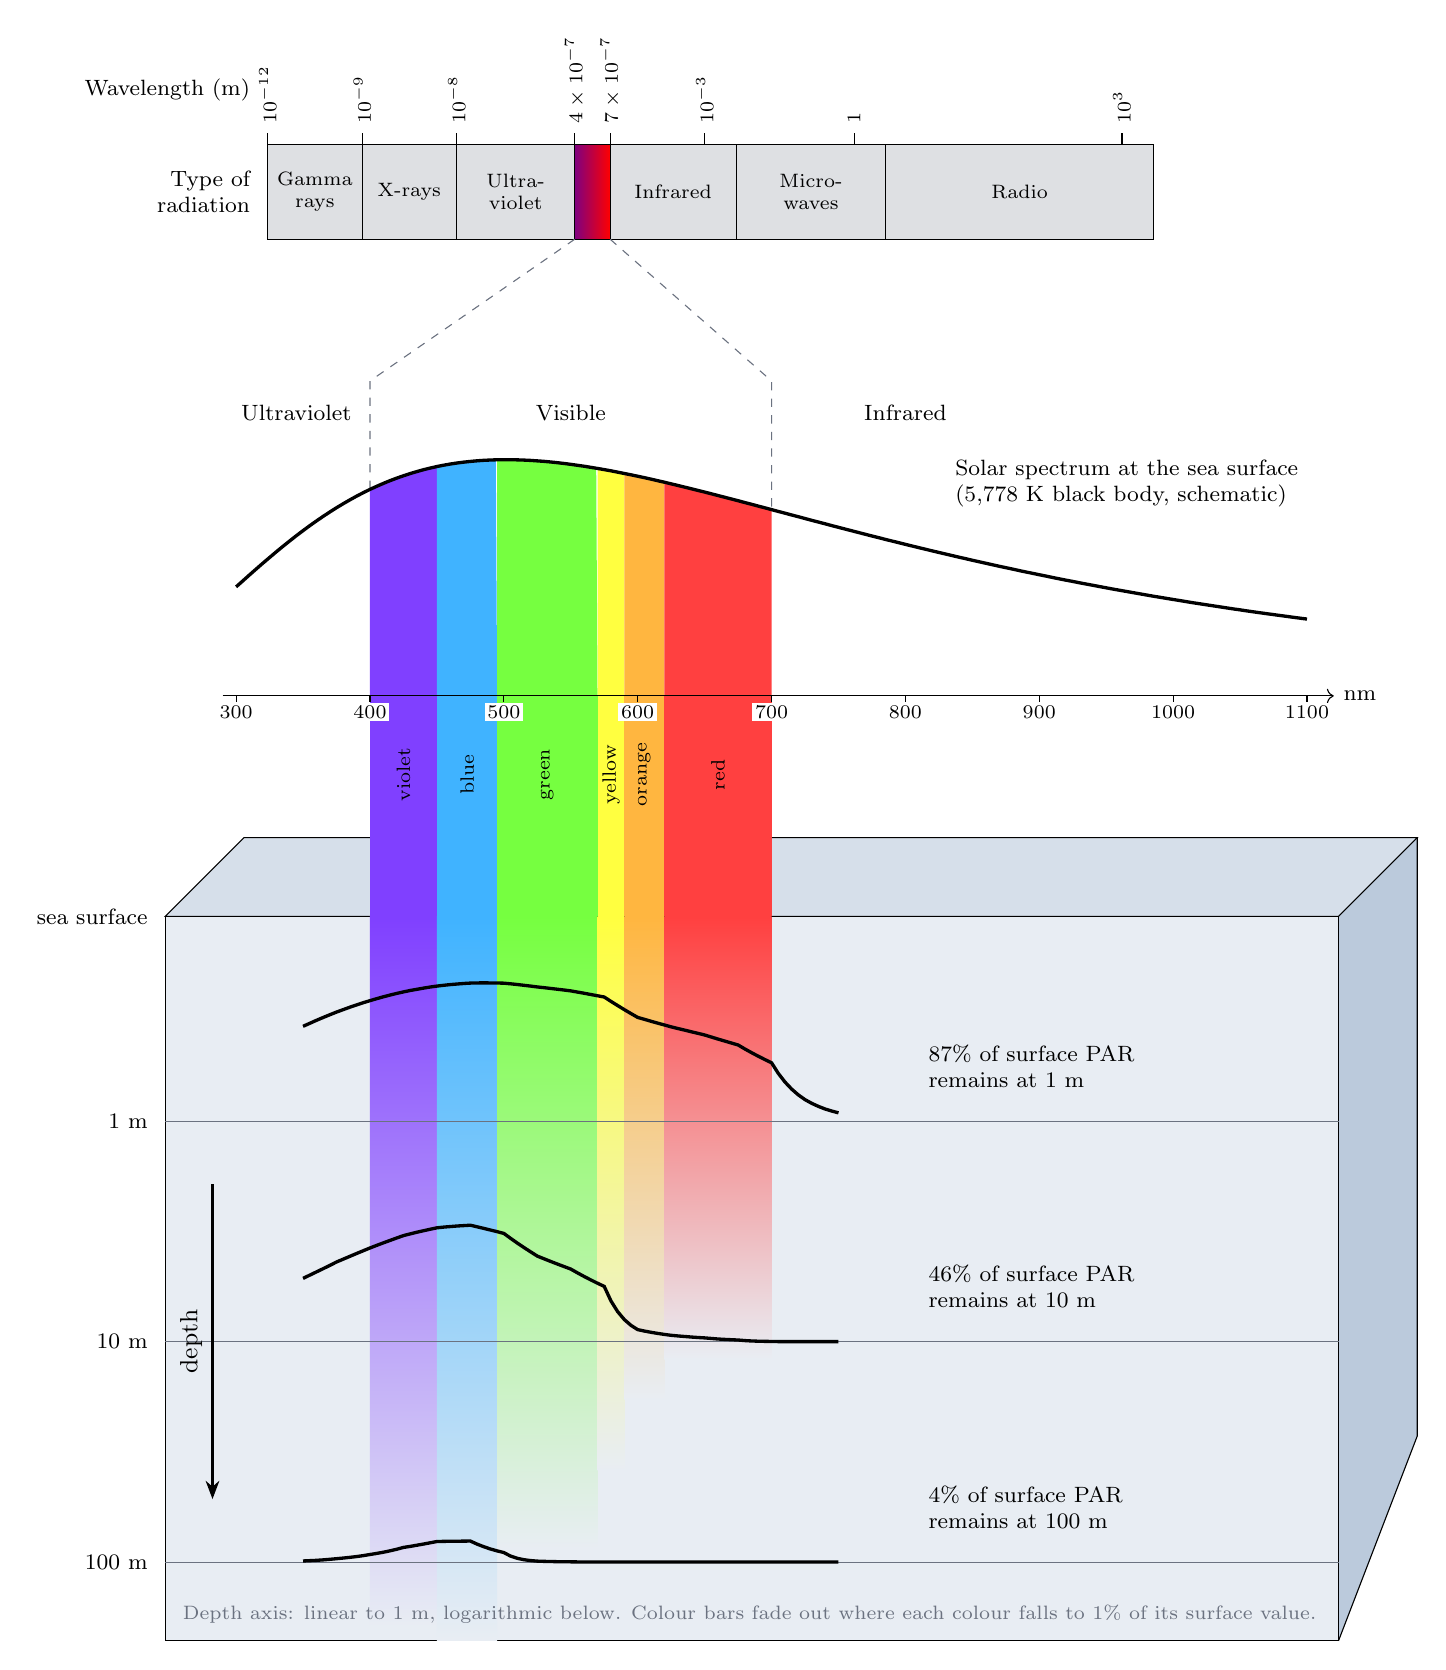
\begin{tikzpicture}[font=\small]
\wavecol{cviolet}{420}
\wavecol{cblue}{470}
\wavecol{cgreen}{530}
\wavecol{cyellow}{580}
\wavecol{corange}{605}
\wavecol{cred}{660}
\node[anchor=east,font=\footnotesize,align=right] at (0.3,11.0) {Type of\\radiation};
\fill[grey!22] (0.4,10.4) rectangle (1.6,11.6); \draw (0.4,10.4) rectangle (1.6,11.6);
\node[font=\scriptsize,align=center,text width=1.0999999999999999cm] at (1.0,11.0) {Gamma\\rays};
\fill[grey!22] (1.6,10.4) rectangle (2.8,11.6); \draw (1.6,10.4) rectangle (2.8,11.6);
\node[font=\scriptsize,align=center,text width=1.0999999999999999cm] at (2.2,11.0) {X-rays};
\fill[grey!22] (2.8,10.4) rectangle (4.3,11.6); \draw (2.8,10.4) rectangle (4.3,11.6);
\node[font=\scriptsize,align=center,text width=1.4cm] at (3.55,11.0) {Ultra-\\violet};
\shade[left color=violet,right color=red] (4.3,10.4) rectangle (4.75,11.6); \draw (4.3,10.4) rectangle (4.75,11.6);
\fill[grey!22] (4.75,10.4) rectangle (6.35,11.6); \draw (4.75,10.4) rectangle (6.35,11.6);
\node[font=\scriptsize,align=center,text width=1.5cm] at (5.55,11.0) {Infrared};
\fill[grey!22] (6.35,10.4) rectangle (8.25,11.6); \draw (6.35,10.4) rectangle (8.25,11.6);
\node[font=\scriptsize,align=center,text width=1.7999999999999998cm] at (7.3,11.0) {Micro-\\waves};
\fill[grey!22] (8.25,10.4) rectangle (11.65,11.6); \draw (8.25,10.4) rectangle (11.65,11.6);
\node[font=\scriptsize,align=center,text width=3.3cm] at (9.95,11.0) {Radio};
\draw (0.4,11.6) -- (0.4,11.75) node[above,rotate=90,anchor=west,font=\scriptsize] {$10^{-12}$};
\draw (1.6,11.6) -- (1.6,11.75) node[above,rotate=90,anchor=west,font=\scriptsize] {$10^{-9}$};
\draw (2.8,11.6) -- (2.8,11.75) node[above,rotate=90,anchor=west,font=\scriptsize] {$10^{-8}$};
\draw (4.3,11.6) -- (4.3,11.75) node[above,rotate=90,anchor=west,font=\scriptsize] {$4\times10^{-7}$};
\draw (4.75,11.6) -- (4.75,11.75) node[above,rotate=90,anchor=west,font=\scriptsize] {$7\times10^{-7}$};
\draw (5.95,11.6) -- (5.95,11.75) node[above,rotate=90,anchor=west,font=\scriptsize] {$10^{-3}$};
\draw (7.85,11.6) -- (7.85,11.75) node[above,rotate=90,anchor=west,font=\scriptsize] {$1$};
\draw (11.25,11.6) -- (11.25,11.75) node[above,rotate=90,anchor=west,font=\scriptsize] {$10^{3}$};
\node[anchor=east,font=\footnotesize] at (0.3,12.3) {Wavelength (m)};
\draw[dashed,grey] (4.3,10.4) -- (1.7000000000000002,8.6) -- (1.7000000000000002,7.2230748451363445); \draw[dashed,grey] (4.75,10.4) -- (6.800000000000001,8.6) -- (6.800000000000001,6.966042186137527);
\node[font=\footnotesize] at (0.765,8.2) {Ultraviolet};
\node[font=\footnotesize] at (4.25,8.2) {Visible};
\node[font=\footnotesize] at (8.5,8.2) {Infrared};
\fill[sea!18] (-0.9,1.8) -- (14.0,1.8) -- (15.0,2.8) -- (0.09999999999999998,2.8) -- cycle;
\fill[sea!30] (14.0,1.8) -- (15.0,2.8) -- (15.0,-4.799999999999999) -- (14.0,-7.3999999999999995) -- cycle;
\fill[sea!10] (-0.9,1.8) rectangle (14.0,-7.3999999999999995);
\draw (-0.9,1.8) -- (14.0,1.8) -- (15.0,2.8) -- (0.09999999999999998,2.8) -- cycle; \draw (-0.9,1.8) rectangle (14.0,-7.3999999999999995); \draw (14.0,-7.3999999999999995) -- (15.0,-4.799999999999999) -- (15.0,2.8);
\node[anchor=east,font=\footnotesize] at (-1.0,1.8) {sea surface};
\fill[cviolet!75] (1.7000000000000002,4.6) -- (1.700,7.223) -- (1.734,7.239) -- (1.768,7.255) -- (1.802,7.270) -- (1.836,7.285) -- (1.870,7.299) -- (1.904,7.314) -- (1.938,7.327) -- (1.972,7.341) -- (2.006,7.354) -- (2.040,7.366) -- (2.074,7.379) -- (2.108,7.390) -- (2.142,7.402) -- (2.176,7.413) -- (2.210,7.424) -- (2.244,7.434) -- (2.278,7.445) -- (2.312,7.454) -- (2.346,7.464) -- (2.380,7.473) -- (2.414,7.481) -- (2.448,7.490) -- (2.482,7.498) -- (2.516,7.505) -- (2.550,7.513) -- (2.5500000000000003,4.6) -- cycle;
\fill[cviolet!75] (1.7000000000000002,1.8) rectangle (2.5500000000000003,4.6);
\node[rotate=90,font=\scriptsize] at (2.125,3.5999999999999996) {violet};
\fill[cblue!75] (2.5500000000000003,4.6) -- (2.550,7.513) -- (2.584,7.520) -- (2.618,7.527) -- (2.652,7.533) -- (2.686,7.539) -- (2.720,7.545) -- (2.754,7.550) -- (2.788,7.555) -- (2.822,7.560) -- (2.856,7.565) -- (2.890,7.569) -- (2.924,7.573) -- (2.958,7.577) -- (2.992,7.580) -- (3.026,7.583) -- (3.060,7.586) -- (3.094,7.589) -- (3.128,7.591) -- (3.162,7.593) -- (3.196,7.595) -- (3.230,7.596) -- (3.264,7.597) -- (3.298,7.598) -- (3.3150000000000004,4.6) -- cycle;
\fill[cblue!75] (2.5500000000000003,1.8) rectangle (3.3150000000000004,4.6);
\node[rotate=90,font=\scriptsize] at (2.9325,3.5999999999999996) {blue};
\fill[cgreen!75] (3.3150000000000004,4.6) -- (3.315,7.599) -- (3.349,7.599) -- (3.383,7.600) -- (3.417,7.600) -- (3.451,7.600) -- (3.485,7.600) -- (3.519,7.599) -- (3.553,7.598) -- (3.587,7.598) -- (3.621,7.596) -- (3.655,7.595) -- (3.689,7.593) -- (3.723,7.592) -- (3.757,7.590) -- (3.791,7.588) -- (3.825,7.585) -- (3.859,7.583) -- (3.893,7.580) -- (3.927,7.577) -- (3.961,7.574) -- (3.995,7.571) -- (4.029,7.567) -- (4.063,7.564) -- (4.097,7.560) -- (4.131,7.556) -- (4.165,7.552) -- (4.199,7.548) -- (4.233,7.543) -- (4.267,7.539) -- (4.301,7.534) -- (4.335,7.529) -- (4.369,7.524) -- (4.403,7.519) -- (4.437,7.514) -- (4.471,7.509) -- (4.505,7.503) -- (4.539,7.498) -- (4.573,7.492) -- (4.590000000000001,4.6) -- cycle;
\fill[cgreen!75] (3.3150000000000004,1.8) rectangle (4.590000000000001,4.6);
\node[rotate=90,font=\scriptsize] at (3.9525000000000006,3.5999999999999996) {green};
\fill[cyellow!75] (4.590000000000001,4.6) -- (4.590,7.489) -- (4.624,7.483) -- (4.658,7.477) -- (4.692,7.471) -- (4.726,7.465) -- (4.760,7.459) -- (4.794,7.452) -- (4.828,7.446) -- (4.862,7.439) -- (4.896,7.432) -- (4.930,7.425) -- (4.930000000000001,4.6) -- cycle;
\fill[cyellow!75] (4.590000000000001,1.8) rectangle (4.930000000000001,4.6);
\node[rotate=90,font=\scriptsize] at (4.760000000000001,3.5999999999999996) {yellow};
\fill[corange!75] (4.930000000000001,4.6) -- (4.930,7.425) -- (4.964,7.418) -- (4.998,7.411) -- (5.032,7.404) -- (5.066,7.397) -- (5.100,7.390) -- (5.134,7.383) -- (5.168,7.375) -- (5.202,7.368) -- (5.236,7.360) -- (5.270,7.353) -- (5.304,7.345) -- (5.338,7.337) -- (5.372,7.329) -- (5.406,7.322) -- (5.440,7.314) -- (5.44,4.6) -- cycle;
\fill[corange!75] (4.930000000000001,1.8) rectangle (5.44,4.6);
\node[rotate=90,font=\scriptsize] at (5.1850000000000005,3.5999999999999996) {orange};
\fill[cred!75] (5.44,4.6) -- (5.440,7.314) -- (5.474,7.306) -- (5.508,7.298) -- (5.542,7.289) -- (5.576,7.281) -- (5.610,7.273) -- (5.644,7.265) -- (5.678,7.257) -- (5.712,7.248) -- (5.746,7.240) -- (5.780,7.231) -- (5.814,7.223) -- (5.848,7.214) -- (5.882,7.206) -- (5.916,7.197) -- (5.950,7.189) -- (5.984,7.180) -- (6.018,7.171) -- (6.052,7.163) -- (6.086,7.154) -- (6.120,7.145) -- (6.154,7.136) -- (6.188,7.127) -- (6.222,7.119) -- (6.256,7.110) -- (6.290,7.101) -- (6.324,7.092) -- (6.358,7.083) -- (6.392,7.074) -- (6.426,7.065) -- (6.460,7.056) -- (6.494,7.047) -- (6.528,7.038) -- (6.562,7.029) -- (6.596,7.020) -- (6.630,7.011) -- (6.664,7.002) -- (6.698,6.993) -- (6.732,6.984) -- (6.766,6.975) -- (6.800,6.966) -- (6.800000000000001,4.6) -- cycle;
\fill[cred!75] (5.44,1.8) rectangle (6.800000000000001,4.6);
\node[rotate=90,font=\scriptsize] at (6.120000000000001,3.5999999999999996) {red};
\draw[very thick] (0.000,5.985) -- (0.085,6.061) -- (0.170,6.137) -- (0.255,6.212) -- (0.340,6.286) -- (0.425,6.358) -- (0.510,6.430) -- (0.595,6.500) -- (0.680,6.568) -- (0.765,6.635) -- (0.850,6.699) -- (0.935,6.762) -- (1.020,6.822) -- (1.105,6.880) -- (1.190,6.936) -- (1.275,6.990) -- (1.360,7.041) -- (1.445,7.090) -- (1.530,7.137) -- (1.615,7.181) -- (1.700,7.223) -- (1.785,7.262) -- (1.870,7.299) -- (1.955,7.334) -- (2.040,7.366) -- (2.125,7.396) -- (2.210,7.424) -- (2.295,7.449) -- (2.380,7.473) -- (2.465,7.494) -- (2.550,7.513) -- (2.635,7.530) -- (2.720,7.545) -- (2.805,7.558) -- (2.890,7.569) -- (2.975,7.578) -- (3.060,7.586) -- (3.145,7.592) -- (3.230,7.596) -- (3.315,7.599) -- (3.400,7.600) -- (3.485,7.600) -- (3.570,7.598) -- (3.655,7.595) -- (3.740,7.591) -- (3.825,7.585) -- (3.910,7.579) -- (3.995,7.571) -- (4.080,7.562) -- (4.165,7.552) -- (4.250,7.541) -- (4.335,7.529) -- (4.420,7.517) -- (4.505,7.503) -- (4.590,7.489) -- (4.675,7.474) -- (4.760,7.459) -- (4.845,7.442) -- (4.930,7.425) -- (5.015,7.408) -- (5.100,7.390) -- (5.185,7.372) -- (5.270,7.353) -- (5.355,7.333) -- (5.440,7.314) -- (5.525,7.293) -- (5.610,7.273) -- (5.695,7.252) -- (5.780,7.231) -- (5.865,7.210) -- (5.950,7.189) -- (6.035,7.167) -- (6.120,7.145) -- (6.205,7.123) -- (6.290,7.101) -- (6.375,7.079) -- (6.460,7.056) -- (6.545,7.034) -- (6.630,7.011) -- (6.715,6.989) -- (6.800,6.966) -- (6.885,6.943) -- (6.970,6.921) -- (7.055,6.898) -- (7.140,6.876) -- (7.225,6.853) -- (7.310,6.830) -- (7.395,6.808) -- (7.480,6.786) -- (7.565,6.763) -- (7.650,6.741) -- (7.735,6.719) -- (7.820,6.697) -- (7.905,6.675) -- (7.990,6.653) -- (8.075,6.631) -- (8.160,6.610) -- (8.245,6.588) -- (8.330,6.567) -- (8.415,6.546) -- (8.500,6.525) -- (8.585,6.504) -- (8.670,6.483) -- (8.755,6.463) -- (8.840,6.442) -- (8.925,6.422) -- (9.010,6.402) -- (9.095,6.382) -- (9.180,6.362) -- (9.265,6.343) -- (9.350,6.323) -- (9.435,6.304) -- (9.520,6.285) -- (9.605,6.266) -- (9.690,6.247) -- (9.775,6.229) -- (9.860,6.211) -- (9.945,6.192) -- (10.030,6.174) -- (10.115,6.157) -- (10.200,6.139) -- (10.285,6.122) -- (10.370,6.104) -- (10.455,6.087) -- (10.540,6.070) -- (10.625,6.054) -- (10.710,6.037) -- (10.795,6.021) -- (10.880,6.005) -- (10.965,5.989) -- (11.050,5.973) -- (11.135,5.957) -- (11.220,5.942) -- (11.305,5.927) -- (11.390,5.912) -- (11.475,5.897) -- (11.560,5.882) -- (11.645,5.867) -- (11.730,5.853) -- (11.815,5.839) -- (11.900,5.825) -- (11.985,5.811) -- (12.070,5.797) -- (12.155,5.783) -- (12.240,5.770) -- (12.325,5.757) -- (12.410,5.744) -- (12.495,5.731) -- (12.580,5.718) -- (12.665,5.705) -- (12.750,5.693) -- (12.835,5.680) -- (12.920,5.668) -- (13.005,5.656) -- (13.090,5.644) -- (13.175,5.633) -- (13.260,5.621) -- (13.345,5.610) -- (13.430,5.598) -- (13.515,5.587) -- (13.600,5.576);
\draw[->] (-0.17,4.6) -- (13.940000000000001,4.6) node[right,font=\footnotesize] {nm};
\draw (0.0,4.6) -- (0.0,4.52) node[below,font=\scriptsize,fill=white,inner sep=1pt] {300};
\draw (1.7000000000000002,4.6) -- (1.7000000000000002,4.52) node[below,font=\scriptsize,fill=white,inner sep=1pt] {400};
\draw (3.4000000000000004,4.6) -- (3.4000000000000004,4.52) node[below,font=\scriptsize,fill=white,inner sep=1pt] {500};
\draw (5.1000000000000005,4.6) -- (5.1000000000000005,4.52) node[below,font=\scriptsize,fill=white,inner sep=1pt] {600};
\draw (6.800000000000001,4.6) -- (6.800000000000001,4.52) node[below,font=\scriptsize,fill=white,inner sep=1pt] {700};
\draw (8.5,4.6) -- (8.5,4.52) node[below,font=\scriptsize,fill=white,inner sep=1pt] {800};
\draw (10.200000000000001,4.6) -- (10.200000000000001,4.52) node[below,font=\scriptsize,fill=white,inner sep=1pt] {900};
\draw (11.9,4.6) -- (11.9,4.52) node[below,font=\scriptsize,fill=white,inner sep=1pt] {1000};
\draw (13.600000000000001,4.6) -- (13.600000000000001,4.52) node[below,font=\scriptsize,fill=white,inner sep=1pt] {1100};
\node[anchor=west,font=\footnotesize,align=left] at (9.01,7.3) {Solar spectrum at the sea surface\\(5,778 K black body, schematic)};
\shade[top color=cviolet!75,bottom color=sea!10] (1.7000000000000002,1.8) rectangle (2.5500000000000003,-7.234);
\shade[top color=cblue!75,bottom color=sea!10] (2.5500000000000003,1.8) rectangle (3.3150000000000004,-7.400);
\shade[top color=cgreen!75,bottom color=sea!10] (3.3150000000000004,1.8) rectangle (4.590000000000001,-6.229);
\shade[top color=cyellow!75,bottom color=sea!10] (4.590000000000001,1.8) rectangle (4.930000000000001,-5.235);
\shade[top color=corange!75,bottom color=sea!10] (4.930000000000001,1.8) rectangle (5.44,-4.333);
\shade[top color=cred!75,bottom color=sea!10] (5.44,1.8) rectangle (6.800000000000001,-3.827);
\draw[grey] (-0.9,-0.8) -- (14.0,-0.8); \node[anchor=east,font=\footnotesize] at (-1.0,-0.8) {1 m};
\draw[very thick] (0.850,0.404) -- (0.935,0.442) -- (1.020,0.480) -- (1.105,0.516) -- (1.190,0.551) -- (1.275,0.585) -- (1.360,0.616) -- (1.445,0.647) -- (1.530,0.676) -- (1.615,0.704) -- (1.700,0.730) -- (1.785,0.755) -- (1.870,0.779) -- (1.955,0.801) -- (2.040,0.822) -- (2.125,0.841) -- (2.210,0.859) -- (2.295,0.874) -- (2.380,0.889) -- (2.465,0.903) -- (2.550,0.915) -- (2.635,0.925) -- (2.720,0.934) -- (2.805,0.941) -- (2.890,0.948) -- (2.975,0.953) -- (3.060,0.955) -- (3.145,0.956) -- (3.230,0.955) -- (3.315,0.954) -- (3.400,0.952) -- (3.485,0.944) -- (3.570,0.935) -- (3.655,0.925) -- (3.740,0.915) -- (3.825,0.904) -- (3.910,0.895) -- (3.995,0.885) -- (4.080,0.875) -- (4.165,0.865) -- (4.250,0.854) -- (4.335,0.839) -- (4.420,0.824) -- (4.505,0.808) -- (4.590,0.792) -- (4.675,0.776) -- (4.760,0.721) -- (4.845,0.668) -- (4.930,0.616) -- (5.015,0.566) -- (5.100,0.517) -- (5.185,0.493) -- (5.270,0.468) -- (5.355,0.444) -- (5.440,0.421) -- (5.525,0.397) -- (5.610,0.376) -- (5.695,0.356) -- (5.780,0.335) -- (5.865,0.315) -- (5.950,0.294) -- (6.035,0.268) -- (6.120,0.242) -- (6.205,0.217) -- (6.290,0.192) -- (6.375,0.167) -- (6.460,0.117) -- (6.545,0.070) -- (6.630,0.025) -- (6.715,-0.018) -- (6.800,-0.059) -- (6.885,-0.193) -- (6.970,-0.303) -- (7.055,-0.393) -- (7.140,-0.467) -- (7.225,-0.527) -- (7.310,-0.574) -- (7.395,-0.613) -- (7.480,-0.646) -- (7.565,-0.672) -- (7.650,-0.695);
\node[anchor=west,font=\footnotesize,align=left] at (8.67,-0.10000000000000009) {87\% of surface PAR\\remains at 1 m};
\draw[grey] (-0.9,-3.6000000000000005) -- (14.0,-3.6000000000000005); \node[anchor=east,font=\footnotesize] at (-1.0,-3.6000000000000005) {10 m};
\draw[very thick] (0.850,-2.797) -- (0.935,-2.756) -- (1.020,-2.715) -- (1.105,-2.674) -- (1.190,-2.632) -- (1.275,-2.589) -- (1.360,-2.553) -- (1.445,-2.517) -- (1.530,-2.481) -- (1.615,-2.446) -- (1.700,-2.411) -- (1.785,-2.378) -- (1.870,-2.346) -- (1.955,-2.315) -- (2.040,-2.284) -- (2.125,-2.254) -- (2.210,-2.232) -- (2.295,-2.211) -- (2.380,-2.192) -- (2.465,-2.173) -- (2.550,-2.155) -- (2.635,-2.146) -- (2.720,-2.139) -- (2.805,-2.132) -- (2.890,-2.127) -- (2.975,-2.122) -- (3.060,-2.142) -- (3.145,-2.162) -- (3.230,-2.183) -- (3.315,-2.204) -- (3.400,-2.226) -- (3.485,-2.288) -- (3.570,-2.348) -- (3.655,-2.405) -- (3.740,-2.460) -- (3.825,-2.514) -- (3.910,-2.548) -- (3.995,-2.582) -- (4.080,-2.615) -- (4.165,-2.647) -- (4.250,-2.679) -- (4.335,-2.727) -- (4.420,-2.773) -- (4.505,-2.817) -- (4.590,-2.859) -- (4.675,-2.899) -- (4.760,-3.083) -- (4.845,-3.219) -- (4.930,-3.320) -- (5.015,-3.394) -- (5.100,-3.448) -- (5.185,-3.466) -- (5.270,-3.482) -- (5.355,-3.496) -- (5.440,-3.509) -- (5.525,-3.520) -- (5.610,-3.528) -- (5.695,-3.535) -- (5.780,-3.542) -- (5.865,-3.548) -- (5.950,-3.553) -- (6.035,-3.560) -- (6.120,-3.567) -- (6.205,-3.572) -- (6.290,-3.576) -- (6.375,-3.580) -- (6.460,-3.587) -- (6.545,-3.592) -- (6.630,-3.595) -- (6.715,-3.597) -- (6.800,-3.598) -- (6.885,-3.600) -- (6.970,-3.600) -- (7.055,-3.600) -- (7.140,-3.600) -- (7.225,-3.600) -- (7.310,-3.600) -- (7.395,-3.600) -- (7.480,-3.600) -- (7.565,-3.600) -- (7.650,-3.600);
\node[anchor=west,font=\footnotesize,align=left] at (8.67,-2.9000000000000004) {46\% of surface PAR\\remains at 10 m};
\draw[grey] (-0.9,-6.3999999999999995) -- (14.0,-6.3999999999999995); \node[anchor=east,font=\footnotesize] at (-1.0,-6.3999999999999995) {100 m};
\draw[very thick] (0.850,-6.386) -- (0.935,-6.382) -- (1.020,-6.378) -- (1.105,-6.372) -- (1.190,-6.365) -- (1.275,-6.357) -- (1.360,-6.349) -- (1.445,-6.340) -- (1.530,-6.330) -- (1.615,-6.318) -- (1.700,-6.304) -- (1.785,-6.290) -- (1.870,-6.275) -- (1.955,-6.257) -- (2.040,-6.237) -- (2.125,-6.214) -- (2.210,-6.201) -- (2.295,-6.186) -- (2.380,-6.171) -- (2.465,-6.155) -- (2.550,-6.139) -- (2.635,-6.137) -- (2.720,-6.136) -- (2.805,-6.135) -- (2.890,-6.134) -- (2.975,-6.133) -- (3.060,-6.172) -- (3.145,-6.205) -- (3.230,-6.234) -- (3.315,-6.258) -- (3.400,-6.279) -- (3.485,-6.324) -- (3.570,-6.352) -- (3.655,-6.370) -- (3.740,-6.381) -- (3.825,-6.388) -- (3.910,-6.391) -- (3.995,-6.393) -- (4.080,-6.395) -- (4.165,-6.396) -- (4.250,-6.397) -- (4.335,-6.398) -- (4.420,-6.399) -- (4.505,-6.399) -- (4.590,-6.400) -- (4.675,-6.400) -- (4.760,-6.400) -- (4.845,-6.400) -- (4.930,-6.400) -- (5.015,-6.400) -- (5.100,-6.400) -- (5.185,-6.400) -- (5.270,-6.400) -- (5.355,-6.400) -- (5.440,-6.400) -- (5.525,-6.400) -- (5.610,-6.400) -- (5.695,-6.400) -- (5.780,-6.400) -- (5.865,-6.400) -- (5.950,-6.400) -- (6.035,-6.400) -- (6.120,-6.400) -- (6.205,-6.400) -- (6.290,-6.400) -- (6.375,-6.400) -- (6.460,-6.400) -- (6.545,-6.400) -- (6.630,-6.400) -- (6.715,-6.400) -- (6.800,-6.400) -- (6.885,-6.400) -- (6.970,-6.400) -- (7.055,-6.400) -- (7.140,-6.400) -- (7.225,-6.400) -- (7.310,-6.400) -- (7.395,-6.400) -- (7.480,-6.400) -- (7.565,-6.400) -- (7.650,-6.400);
\node[anchor=west,font=\footnotesize,align=left] at (8.67,-5.699999999999999) {4\% of surface PAR\\remains at 100 m};
\draw[-{Stealth},thick] (-0.30000000000000004,-1.5999999999999999) -- (-0.30000000000000004,-5.6000000000000005) node[midway,left,rotate=90,anchor=south] {depth};
\node[font=\scriptsize,grey,anchor=south west] at (-0.8,-7.3) {Depth axis: linear to 1 m, logarithmic below. Colour bars fade out where each colour falls to 1\% of its surface value.};
\end{tikzpicture}\end{document}